\documentclass[10pt,spanish,a4paper,openany,notitlepage]{article}
%-------------------------------------Paquetes-----------------------------------------------------------------------
\usepackage[spanish,es-tabla]{babel}  	% Traduce los textos a castellano
\usepackage[utf8]{inputenc}	% Permite escribir directamente áéíóúñ
\usepackage{t1enc}            	% Agrega caracteres extendidos al font
\usepackage{amsmath} 		%Permite imprimir mas opcciones matematicas
\usepackage{graphicx}		%Permite agregar imagenes al informe
\usepackage{multicol}  		%Permite dividir el texto en varias columnas
\usepackage{float} 		%Permite utilizar H para colocar las imagenes en un lugar especifico 
\usepackage{units}
\usepackage{circuitikz}
\usepackage{caption}
\usepackage{subcaption}
\usepackage{sidecap}
\usepackage{mathtools}
\usepackage{multirow} % Paquete para dividir las tablas en subtablas
\usepackage{booktabs} %estos 2 sirven para achicar la tabla
\usepackage{tabulary}
\usepackage{fancyhdr} % encabezado
\usepackage{textcomp} % para usar ° con el comando \textdegree
\usepackage{anysize}		%Permite modificar los margenes del documento
\usepackage{abstract} % paquete para el resumen del articulo
\usepackage{amssymb}
\usepackage{makecell}
\usepackage{listings}
\lstset{
	language=Octave,
	morecomment = [l][\itshape\color{blue}]{\%}
}

%---------------------------------------Configuraciones de pagina----------------------------------------------
\marginsize{2.5cm}{2.5cm}{1cm}{1cm}

\pagestyle{fancy}
\fancyhf{}
\lhead{
86.05 - \textsc{Señales y Sistemas}\\ 
2\textsuperscript{do} Cuatrimestre de 2015
}
\rhead{
\includegraphics[width=3cm]{imagenes/FIUBA_ALTA.jpg}}
\rfoot{Página \thepage}

%---------------------------------------Definiciones propias---------------------------------------------------------
\newcommand{\oiint}{\displaystyle\bigcirc\!\!\!\!\!\!\!\!\int\!\!\!\!\!\int} %Integral doble cerrada

\DeclarePairedDelimiter\abs{\lvert}{\rvert}%
\DeclarePairedDelimiter\norm{\lVert}{\rVert}%
% Swap the definition of \abs* and \norm*, so that \abs
% and \norm resizes the size of the brackets, and the 
% starred version does not.
\makeatletter
\let\oldabs\abs
\def\abs{\@ifstar{\oldabs}{\oldabs*}}
%
\let\oldnorm\norm
\def\norm{\@ifstar{\oldnorm}{\oldnorm*}}
\makeatother
%--------------------------------------------------------------------------------------------------------------------------------


\makeatletter
\let\ps@plain\ps@fancy 
\makeatother

% lo siguiente es para borrar el titulo del resumen y que no ocupe espacio:
 \AtBeginDocument{%
 \renewcommand{\abstractname}{}%
 }
\renewcommand{\absnamepos}{empty} % originally center
 

\begin{document}
\title{\textbf{Proyecto Especial: Reconocimiento de audio mediante huellas digitales acústicas}}
\author{
  Vázquez, Matías - 91523\\
  \texttt{mfvazquez@gmail.com}
}
\date{\today}
\maketitle

\begin{abstract} %Resumen
\emph{En este trabajo se implementará un software de reconocimiento
de canciones mediante huellas digitales acústicas en Octave. Para su desarrollo
se hará uso de técnicas y herramientas de análisis de señales; 
DFT, espectrogramas, diseño de filtros digitales y cambio de la tasa
de muestreo.}
\end{abstract}

\section{Introducción}

\subsection{Reconocimiento mediante huellas digitales acústicas}

El reconocimiento de audio mediante huellas digitales acústicas es una técnica que busca
identificar una pieza de audio, contrastando la información contenida en dicha pieza contra
la almacenada en una base de datos de pistas conocidas.

Existen varias formas de abordar el problema del reconocimiento, pero todas persiguen la
misma finalidad:

\begin{itemize}
\item Simplicidad computacional: el reconocimiento debe realizarse en forma rápida.
\item Ser eficiente en el uso de memoria y poseer buena capacidad de discriminación
\item Ser robusto ante distorsiones: ruido de fondo, degradación por compresión digital del
audio, ecualización por respuesta en frecuencia no plana del lugar y/o parlantes, etc.
\item Granularidad: capacidad de reconocimiento utilizando solo un segmento del audio.
\item Alta tasa de aciertos, baja tasa de falsos positivos y de rechazos.
\end{itemize}

El procedimiento básico consiste en analizar el segmento de audio, buscando extraer
características particulares en el espacio tiempo-frecuencia (es decir, en su espectrograma)
que sirvan para identificarlo luego. Una característica podría ser, por ejemplo, la potencia
que posean las diferentes bandas de frecuencias. Al conjunto de estas características se las
denomina huella digital acústica , ya que es análogo a como una huella dactilar se identifica
por las convergencias, desviaciones, interrupciones y demás particularidades de las crestas
papilares.

\begin{figure}[H] %[h] para here [b] para bottom [t] para top [H]+float para aqui si o si
\begin{center}
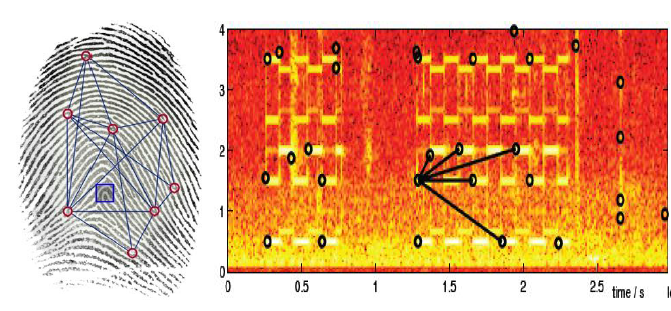
\includegraphics[scale=0.7]{./imagenes/huella.png}
\caption{Analogía entre una huella digital tradicional y una huella digital acústica}
 \label{fig:ej_huella}
\end{center}
\end{figure}

Este procedimiento de extracción de huellas se utiliza tanto para confeccionar la base de
datos de canciones conocidas como para posteriormente reconocer segmentos de audio sin
identificar, consultando la base de datos.

La elección de las características es la base del funcionamiento del método, ya que serán
las claves que se utilizan luego para realizar la búsqueda en la base de datos. Por lo tanto,
deben ser lo suficientemente específicas como para identificar a cada canción
unívocamente, pero a la vez ocupar poca memoria para permitir realizar la búsqueda en
forma rápida y eficiente. También deberán ser relativamente inmunes ante ruidos y
distorsiones del audio, de manera de lograr un sistema de reconocimiento robusto.

En este trabajo se desarrollará una implementación que utiliza como características el
signo de la diferencia de energía entre bandas, también conocido como algoritmo Philips.

Cabe destacar que este y los algoritmos antes mencionados sólo reconocen las mismas
versiones de las canciones que se almacenan en la base de datos, es decir, no están
diseñados para reconocer versiones en vivo o interpretaciones diferentes a la original.

\subsection{Descripción del sistema de reconocimiento}

El sistema de reconocimiento consta de dos bloques principales:

\begin{enumerate}
\item El algoritmo para extraer las huellas digitales acústicas.
\item La base de datos que almacena las huellas acústicas de las canciones conocidas
y permite realizar búsquedas a partir de la huella acústica de una canción
desconocida.
\end{enumerate}

El algoritmo para extraer las huellas acústicas toma como entrada el canal de audio y,
luego de un preprocesamiento de la señal, extrae las características y entrega como
resultado la huella acústica. El proceso se esquematiza a continuación:

\begin{figure}[H] %[h] para here [b] para bottom [t] para top [H]+float para aqui si o si
\begin{center}
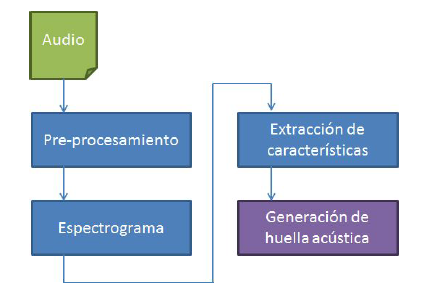
\includegraphics[scale=0.8]{./imagenes/extraccion.png}
\caption{Esquema del algoritmo para extraer la huella digital acústica}
 \label{fig:extraccion}
\end{center}
\end{figure}

La base de datos guardará las huellas acústicas de las canciones conocidas. Tiene además
un sistema de búsqueda tal que al realizar un query con una huella acústica dada 
nos devuelve la canción más probable a la cual corresponde.

El esquema del sistema completo se presenta a continuación:

\begin{figure}[H] %[h] para here [b] para bottom [t] para top [H]+float para aqui si o si
\begin{center}
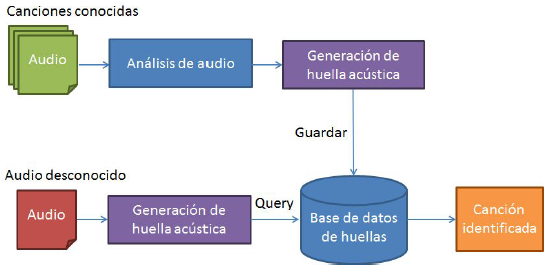
\includegraphics[scale=0.8]{./imagenes/esquema.png}
\caption{Esquema representando la generación de la base de datos de huellas acústicas y la consulta.}
 \label{fig:esquema}
\end{center}
\end{figure}

\section{Pre-procesamiento del audio}

El pre-procesamiento del audio consiste en pasarlo a canal mono (si
está en estéreo) y luego submuestrearlo, debido a que la información
útil para la extracción de características se encuentra en bajas frecuencias.
En general, el audio está muestreado a $44100\, \unit{Hz}$ (calidad de CD).
Para este algoritmo basta con tenerlo muestreado a 1/8 de su frecuencia original,
es decir $5512.5\, \unit{Hz}$. Esto permite trabajar con menos muestras, aliviando la
carga computacional.

\subsection{Obtención de la pista de audio}

Mediante la función \texttt{audioread} se cargó la pista de audio.
Si el audio cargado es una matriz de 2 columnas, cada columna corresponde
a un canal de audio, se promedian los canales utilizando la función
\texttt{mean} para tener 1 solo canal.
En la figura \ref{fig:Ej1_audio} se muestra una porción de la señal resultante.

\begin{figure}[H] %[h] para here [b] para bottom [t] para top [H]+float para aqui si o si
\begin{center}
\includegraphics[scale=0.6]{../Imagenes/Ej1_canal.png}
\caption{Porción de la pista de audio.}
 \label{fig:Ej1_audio}
\end{center}
\end{figure}

\subsection{Análisis espectral de la señal}

Se realizó la FFT del canal de audio, para luego obtener la densidad
espectral de potencia. La densidad espectral de potencia $S_{xx}$
se define como:

\begin{equation}
S_{xx}(w) = |X(w)|^2
\end{equation}

donde $X(w)$ es la transformada de Fourier del canal de audio.
Para pasarla a escala logarítmica se utilizó la siguiente ecuación:

\begin{equation}
P_{xx} = 10 log_{10}(S_{xx}(w))
\label{eq:pot_log}
\end{equation}

La estimación de la densidad espectral mejora si se divide el audio
en segmentos y promedia (en potencia) el espectro de cada segmento.
Por lo que se utilizó la función \texttt{specgram}\footnote{Se utilizó esta
función en lugar de \texttt{fft} ya que realiza de forma
más eficiente la obtención de la FFT del canal, además
de que utiliza menos memoria ya que solo retorna las frecuencias
entre 0 y $\pi$ a diferencia de la \texttt{fft} que devuelve
las frecuencias entre 0 y $2\pi$.
}, con una longitud de ventana de 256 y overlap 0, para luego obtener
su densidad espectral de potencia mediante la ecuación \ref{eq:pot_log} y finalmente
promediarla en tiempo. 
En la figura \ref{fig:Ej2_pot} se muestra el resultado obtenido, como
se puede observar la mayor densidad de potencia se encuentra en las bajas frecuencias.
Para frecuencias superiores a los $2.5\, \unit{KHz}$ la densidad
espectral de potencia se encuentra por debajo de los $0\, \unit{dB}$. 

\begin{figure}[H] %[h] para here [b] para bottom [t] para top [H]+float para aqui si o si
\begin{center}
\includegraphics[scale=0.6]{../Imagenes/Ej2_densidad_frecuencias.png}
\caption{Densidad espectral de potencia del canal de audio.}
 \label{fig:Ej2_pot}
\end{center}
\end{figure}

\subsection{Reducción de la frecuencia de muestreo}

Se implementó un sistema para reducir la frecuencia de muestreo del audio
de $44100\, \unit{Hz}$ a $5512.5\, \unit{Hz}$. En la figura \ref{fig:filtro_bloque}
se muestra el diagrama en bloques del sistema.
Primero se filtra la señal con un filtro pasabajos, para evitar el aliasing
al submuestrear la señal. Ya que si se reduce la frecuencia de muestreo a
$5512.5\, \unit{Hz}$ debemos filtrar las frecuencias mayores o iguales 
$\frac{5512.5}{2}\, \unit{Hz} = 2756.25\, \unit{Hz}$.


\begin{figure}[H] %[h] para here [b] para bottom [t] para top [H]+float para aqui si o si
\begin{center}
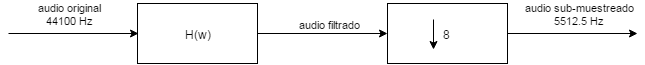
\includegraphics[scale=0.8]{./imagenes/filtro_bloque.png}
\caption{Diagramas en bloques del sistema.}
 \label{fig:filtro_bloque}
\end{center}
\end{figure}

Para el diseño del filtro pasa-bajos se impusieron las siguientes condiciones:

\begin{itemize}
\item Fase lineal
\item Retardo menor a $1\, \unit{ms}$
\end{itemize}

Como la Fase debe ser lineal se optó por utilizar filtros tipo FIR,
ya que los filtros IIR no tienen fase lineal a diferencia de los FIR.

Para garantizar un retardo menor a $1\, \unit{ms}$ el orden del filtro
debe ser menor o igual a 88, ya que para ordenes superiores el retardo
será mayor a $1\, \unit{ms}$.

Se utilizó una ventana de Hamming de orden 88 para el filtro, ya que presenta
una mejor atenuación en las frecuencias superiores a la frecuencia de
corte, a diferencia de la ventana rectangular. Con una frecuencia de
corte de $1750\, \unit{Hz}$. Se eligió una frecuencia de corte
menor a los $2756.25\, \unit{Hz}$ debido a que el filtro no es ideal
y a que no puede tener un orden superior a 88.

Mediante la función \texttt{zplane} se obtuvo el
diagrama de polos y ceros mostrado en la figura \ref{fig:polos_y_ceros} 

\begin{figure}[H] %[h] para here [b] para bottom [t] para top [H]+float para aqui si o si
\begin{center}
\includegraphics[scale=0.8]{../Imagenes/Ej3_polos_y_ceros.png}
\caption{Diagrama de polos y ceros}
 \label{fig:polos_y_ceros}
\end{center}
\end{figure}

Mediante la funcion \texttt{freqz} se obtuvo la
respuesta en frecuencia mostrada en la figura \ref{fig:resp_frec}.

\begin{figure}[H] %[h] para here [b] para bottom [t] para top [H]+float para aqui si o si
\begin{center}
\includegraphics[scale=0.6]{../Imagenes/Ej3_respuesta_en_frecuencia.png}
\caption{Respuesta en frecuencia}
 \label{fig:resp_frec}
\end{center}
\end{figure}

Mediante la funcion \texttt{impz} se obtuvo la
respuesta al impulso mostrada en la figura \ref{fig:resp_imp}.

\begin{figure}[H] %[h] para here [b] para bottom [t] para top [H]+float para aqui si o si
\begin{center}
\includegraphics[scale=0.6]{../Imagenes/Ej3_respuesta_al_impulso.png}
\caption{Respuesta al impulso}
 \label{fig:resp_imp}
\end{center}
\end{figure}

Mediante la funcion \texttt{grpdelay} se obtuvo la
respuesta en frecuencia mostrada en la figura \ref{fig:retardo}.
Siendo el retardo de grupo de $997.732\, \unit{\mu s}$

\begin{figure}[H] %[h] para here [b] para bottom [t] para top [H]+float para aqui si o si
\begin{center}
\includegraphics[scale=0.6]{../Imagenes/Ej3_retardo_de_grupo.png}
\caption{Retardo de grupo}
 \label{fig:retardo}
\end{center}
\end{figure}

\subsection{Espectrogramas de la señal original y la filtrada}

Mediante la función \texttt{specgram}, con una ventana de Hamming de longitud
256 y overlap del $50\, \unit{\%}$, se obtuvieron los espectrogramas
del canal de audio(figura \ref{fig:espectrograma_original}) y del
canal de audio luego ser filtrado (figura \ref{fig:espectrograma_filtrado}).
Como puede observarse en el espectrograma de la señal filtrada, para
frecuencias superiores a los $2.5\, \unit{KHz}$ la potencia se encuentra
alrededor de los $-50\, \unit{dB}$.


\begin{figure}[H] %[h] para here [b] para bottom [t] para top [H]+float para aqui si o si
\begin{center}
\includegraphics[scale=0.6]{../Imagenes/Ej4_espectrograma_original.png}
\caption{Espectrograma del canal de audio}
 \label{fig:espectrograma_original}
\end{center}
\end{figure}

\begin{figure}[H] %[h] para here [b] para bottom [t] para top [H]+float para aqui si o si
\begin{center}
\includegraphics[scale=0.6]{../Imagenes/Ej4_espectrograma_filtrado.png}
\caption{Espectrograma del canal de audio filtrado}
 \label{fig:espectrograma_filtrado}
\end{center}
\end{figure}

\subsection{Comparación entre ventana rectangular y Hamming}

Mediante la función \texttt{fft} se obtuvo el espectro de una
ventana rectangular y una de Hamming, ambas de duración 26.
En la figura \ref{fig:rec_vs_hamm} se graficó la potencia de ambas ventanas
en escala logarítmica en un mismo gráfico para compararlos, con una
separación entre los puntos del gráfico de $70\, \unit{Hz}$ por lo que
la resolución es $\frac{44100\,\unit{Hz}}{70\,\unit{Hz}} = 630$.

\begin{figure}[H] %[h] para here [b] para bottom [t] para top [H]+float para aqui si o si
\begin{center}
\includegraphics[scale=0.6]{../Imagenes/Ej5_comparacion_ventanas.png}
\caption{Potencia en escala logaritmica del espectro de una ventana rectangular y Hamming}
 \label{fig:rec_vs_hamm}
\end{center}
\end{figure}

Como puede observarse en la figura la ventana de Hamming cuenta
con una mayor atenuación en sus lóbulos secundarios a comparación
de la ventana rectangular, esto es importante ya que al utilizarla
para realizar espectrogramas se va a obtener menos solapamiento que utilizando
la ventana rectangular. También puede observarse que el lóbulo principal
de Hamming tiene un ancho mayor al de la rectangular.

\subsection{Comparación de espectrogramas con diferentes ventanas}

Se realizaron espectrogramas de la señal submuestreada con ventana
rectangular y Hamming, con 3 longitudes de ventana diferentes para
cada ventana.

A continuación se muestran, para los dos tipos de ventana utilizadas,
los espectrogramas con longitudes de 64, 4096 y 8192\footnote{se eligieron 
estas longitudes de ventana para aprovechar la eficacia de la FFT ante longitudes que son potencias de 2}
y overlap del $50\,\unit{\%}$. 
Se hizo un zoom entre los $60\, \unit{s}$ y $80\, \unit{s}$ del audio.

Espectrogramas usando ventana rectangular:

\begin{figure}[H] %[h] para here [b] para bottom [t] para top [H]+float para aqui si o si
\begin{center}
\includegraphics[scale=0.5]{../Imagenes/Ej6_espetrograma_rectangular_N=64.png}
\caption{Espectrograma de la señal submuestreada con ventana rectangular de longitud 64}
 \label{fig:rec_N=64}
\end{center}
\end{figure}

\begin{figure}[H] %[h] para here [b] para bottom [t] para top [H]+float para aqui si o si
\begin{center}
\includegraphics[scale=0.5]{../Imagenes/Ej6_espetrograma_rectangular_N=4096.png}
\caption{Espectrograma de la señal submuestreada con ventana rectangular de longitud 4096}
 \label{fig:rec_N=4096}
\end{center}
\end{figure}

\begin{figure}[H] %[h] para here [b] para bottom [t] para top [H]+float para aqui si o si
\begin{center}
\includegraphics[scale=0.5]{../Imagenes/Ej6_espetrograma_rectangular_N=8192.png}
\caption{Espectrograma de la señal submuestreada con ventana rectangular de longitud 8192}
 \label{fig:rec_N=8192}
\end{center}
\end{figure}

Espectrogramas usando ventana Hamming:

\begin{figure}[H] %[h] para here [b] para bottom [t] para top [H]+float para aqui si o si
\begin{center}
\includegraphics[scale=0.5]{../Imagenes/Ej6_espetrograma_hamming_N=64.png}
\caption{Espectrograma de la señal submuestreada con ventana Hamming de longitud 64}
 \label{fig:hamm_N=64}
\end{center}
\end{figure}

\begin{figure}[H] %[h] para here [b] para bottom [t] para top [H]+float para aqui si o si
\begin{center}
\includegraphics[scale=0.5]{../Imagenes/Ej6_espetrograma_hamming_N=4096.png}
\caption{Espectrograma de la señal submuestreada con ventana Hamming de longitud 4096}
 \label{fig:hamm_N=4096}
\end{center}
\end{figure}

\begin{figure}[H] %[h] para here [b] para bottom [t] para top [H]+float para aqui si o si
\begin{center}
\includegraphics[scale=0.5]{../Imagenes/Ej6_espetrograma_hamming_N=8192.png}
\caption{Espectrograma de la señal submuestreada con ventana Hamming de longitud 8192}
 \label{fig:hamm_N=8192}
\end{center}
\end{figure}

Como puede observarse en los espectrogramas, a medida que aumenta
la longitud de la ventana, disminuye la resolución en tiempo pero aumenta
la resolución en frecuencia. De forma inversa a medida que disminuye la longitud de
la ventana, aumenta la resolución en tiempo pero disminuye la resolución
en frecuencia.

Comparando los espectrogramas entre diferentes ventanas, podemos observar
que con ventana Hamming se obtuvieron valores mas precisos. Esto se puede
notar en las frecuencias altas, en la ventana rectangular se nota como
la potencia de un segmento es influida por la potencia en los segmentos
adyacentes. Esto se debe a que los lóbulos secundarios de la ventana
rectangular tienen mayor amplitud que los de la ventana de Hamming, por
lo que el solapamiento termina influyendo en el resultado.

Esto puede observarse mejor en las siguientes figuras con un zoom ahora
en frecuencias entre $1500\, \unit{Hz}$ y $2756.25\, \unit{Hz}$.

\begin{figure}[H] %[h] para here [b] para bottom [t] para top [H]+float para aqui si o si
\begin{center}
\includegraphics[scale=0.5]{../Imagenes/Ej6_espetrograma_hamming_zoom.png}
\caption{Espectrograma de la señal submuestreada con ventana Hamming de longitud 64}
 \label{fig:hamm_zoom}
\end{center}
\end{figure}

\begin{figure}[H] %[h] para here [b] para bottom [t] para top [H]+float para aqui si o si
\begin{center}
\includegraphics[scale=0.5]{../Imagenes/Ej6_espetrograma_rectangular_zoom.png}
\caption{Espectrograma de la señal submuestreada con ventana rectangular de longitud 64}
 \label{fig:rect_zoom}
\end{center}
\end{figure}

Como se puede observar en el espectrograma con ventana rectangular(figura \ref{fig:rect_zoom})
en las zonas con mayor densidad de potencia alcanza valores cercanos
a los $0\, \unit{dB}$. En cambio para el espectrograma con ventana Hamming
(figura \ref{fig:hamm_zoom}) en las mismas zonas alcanza valores de 
aproximadamente $-30\, \unit{dB}$.

Para el algoritmo se utilizará una ventana Hamming de longitud 2048.

\section{Extracción de características del espectrograma}

Para el algoritmo, las características se obtuvieron mediante una función signo $ F(m,n)$
que opera sobre la energía de las bandas de frecuencia $E(m,n)$  según:\\

\begin{equation}
F(m,n)= \left\{ \begin{array}{lcc}
             1 &   si  & E(m,n) - E(m+1,n) > E(m,n-1) - E(m+1,n-1) \\
             \\0 &  & en\ otro\ caso \\
             \end{array}
   \right.
\end{equation}

$n$ es el tiempo y $m$ la banda de frecuencia. Se comprueba que F $(m,n)$ es 1 si la diferencia de
energía entre las bandas $m$ y $ m+1$ para el frame actual $n$ es mayor a la del frame anterior
$n-1$.

Las bandas de frecuencia se definieron con espaciamiento logarítmico (esto es similar a la escala
psicoacústica Bark) debido a que el oído diferencia el espaciamiento entre tonos en forma
logarítmica.

\subsection{Implementación del algoritmo}

En el apendice \ref{codigo:caracteristicas} se encuentra el codigo
del algoritmo de extracción de características.

Para dividir el espectrograma en 21 bandas de frecuencia espaciadas
logaritmicamente se utilizó la funcion \texttt{logspace} para generar
un vector de 22 elementos separados logaritmicamente iniciando en $300\, \unit{Hz}$
y finalizando en $2000\, \unit{Hz}$.
Luego se recorrió el vector de frecuencias y se fueron tomando las primeras
frecuencias que se encontraban entre los segmentos de frecuencias del vector
generado. Descartando las demas frecuencias no seleccionadas.
En el apéndice \ref{codigo:generar_huella} se encuentra el cogido de la
función que genera las huellas.

En la figura \ref{fig:huella} se ve una huella de un segmento de audio.

\begin{figure}[H] %[h] para here [b] para bottom [t] para top [H]+float para aqui si o si
\begin{center}
\includegraphics[scale=0.5]{../Imagenes/Ej7_huella.png}
\caption{Huella de un segmento de audio}
 \label{fig:huella}
\end{center}
\end{figure}


\section{Confección de la base de datos}

La base de datos es una tabla de $2^{20}$ filas y $N$ columnas. Para cada frame de la huella
acústica, se genera un valor a guardar en la tabla. La fila en la que se guarda cada valor se
obtiene pasando a decimal el número binario conformado por las características del frame
en cuestión, y la columna en la que se guarda se elige buscando la última columna vacía
dentro de esa fila. Note que la cantidad de filas de la tabla es debido a que cada frame de la
huella acústica posee 20 elementos binarios.
Cada valor a guardar es un entero de 32 bits, de los cuales los 12 bits menos significativos
son el ID numérico de la canción que se está analizando, y los 20 más significativos el
número del frame. Observe que el máximo número de canciones distintas que se podrán
almacenar en esta tabla es $2^{12}$.

\begin{figure}[H] %[h] para here [b] para bottom [t] para top [H]+float para aqui si o si
\begin{center}
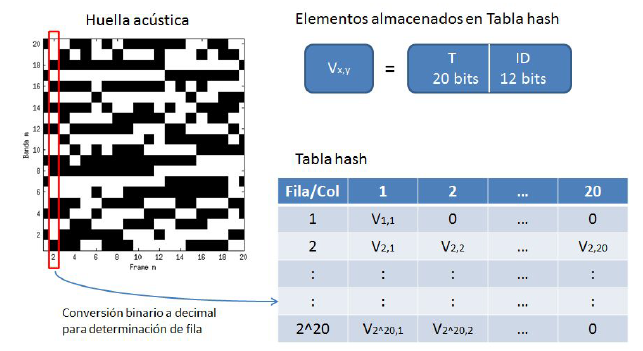
\includegraphics[scale=0.8]{./imagenes/bd.png}
\caption{Indexación de tabla hash mediante huella acústica y representación de elementos almacenados.}
 \label{fig:bd}
\end{center}
\end{figure}

Para el frame número 2 (recuadrado en rojo) la característica en binario es
11010101011001100110. Pasando este número a decimal obtenemos la fila de la tabla
en la que deberá guardarse el valor. Supongamos que la huella corresponde a una canción
con ID=5, entonces el elemento a almacenar será, en binario:
V=[00000000000000000010 000000000101].

\subsection{Script para generar la base de datos}

Para generar la base de datos se utilizó el script del apéndice \ref{codigo:generar_DB}
el cual lee todos los archivos con formato \texttt{wav} del directorio \texttt{../Musica/}.
Utiliza la función que genera huellas acústicas directamente de un archivo, ver
apendice \ref{codigo:generar_huella_arch}.

La base de datos junto a un vector con los nombres de los archivos
que la componen son guardadas en un archivo con formato \texttt{mat}.
El vector con los nombres de los archivos es utilizado para poder
leer su información cuando se desee identificar un fragmento de audio.

\subsection{Solapamiento entre ventanas del espectrograma}

Se calculó un solapamiento de ventanas del espectrograma para
obtener una densidad de aproximadamente 25 elementos por segundo.

Como se mencionó antes, el largo de las ventanas es de 2048. El audio
cuenta con 5512.5 elementos por segundo. Por lo que se calculó la
distancia entre ventanas mediante:

\[ \displaystyle distancia = \frac{5512.5}{25} = 220.5 \]

Luego el solapamiento entre ventanas se calcula restándole a la longitud
de la ventana la distancia entre ventanas:

\[ \displaystyle N_{overlap} = 2048 - 220.5 = 1827.5 \]

Como $N_{overlap}$ debe ser entero, se redondeó el valor utilizando
la función \texttt{ceil} quedando el siguiente resultado final:

\[ \displaystyle N_{overlap} = 1828 \]

\section{Test del algoritmo}

En esta etapa, se puso a prueba la eficacia del algoritmo completo
de reconocimiento. El procedimiento consistirá en obtener el porcentaje
de aciertos del método al reconocer segmentos de audio, los cuales fueron
sometidos a distintas distorsiones.

En los apéndices \ref{codigo:rendimiento} y \ref{codigo:tests} puede
verse el código utilizado para realizar las pruebas de esta sección.

Para todas las pruebas se analizaron dos tipos de aciertos. Como el algoritmo
devuelve 5 posibles canciones con orden de prioridad descendente, se analizó 
la tasa de aciertos cuando la canción figura en el primer puesto y para 
cuando la canción se encuentra entre los primeros 5 puestos.

\subsection{Tasa de aciertos para segmentos de distintas duraciones}
\label{section:test}

Se evaluó la tasa de aciertos del algoritmo identificando segmentos
de duración T con tiempo inicial elegido al azar de canciones elegidas
al azar. Las canciones son las mismas que se utilizaron para generar
la base de datos. Se realizó la evaluación para 50 segmentos con
duración $T$ entre 5, 10 y 20 segundos cada vez(150 evaluaciones en total)
obteniendo la tasa de aciertos en cada caso.

\begin{table}[H]
\centering
\begin{tabular}{|c|c|c|}
\hline
$T \unit{[s]}$ & Aciertos en primer puesto & Acierto entre primeros 5 \\
\hline
$5$ & 50 & 50\\
\hline
$10$ & 50 & 50\\
\hline
$20$ & 50 & 50\\
\hline
\end{tabular}
\caption{Aciertos para distintos intervalos de tiempo}
\label{table:segmentos}
\end{table}

Como se ve en la tabla \ref{table:segmentos} se obtuvo
una tasa de aciertos del $100\,\unit{\%}$ para todas las evaluaciones.

\subsection{Prueba identificando audios grabados}

Se realizó una prueba intentando identificar una canción reproducida
de unos parlantes de una computadora, y grabados con un micrófono conectado
a la computadora. Para esta prueba la duración del audio fue de 15 segundos
y el audio grabado tenia un nivel de volumen mas bajo que el original.
El algoritmo logró identificar la canción en el primer puesto de los resultados.

Luego se realizó otra prueba reproduciendo una canción desde el parlante
de un celular y grabándolo con el micrófono que viene integrado a una notebook.
La duración del audio grabado era de 30 segundos, el volumen del audio
era mas bajo que el original.
El algoritmo no logró identificar la canción en el primer puesto de los
resultados, la canción se encontraba en el segundo puesto.
Esto se debe a que los parlantes de los celulares en general son de baja
calidad y suelen comportarse como un filtro pasa alto. Si tiene
una frecuencia de corte superior a los $300\,\unit{Hz}$ el algoritmo
no devolverá valores acertados ya que esas frecuencias son las que
influyen más en la identificación del audio, debido a la escala logaritmica
en frecuencia.

\subsection{Tasa de aciertos agregando ruido}

Se repitió las pruebas de la sección \ref{section:test} pero agregando
distintas intensidades de ruido a los segmentos de audio; SNR $0\,\unit{dB}$,
$10\,\unit{dB}$ y $20\,\unit{dB}$.

Se obtuvo la relación entre la potencia del ruido y la del audio para
cada SNR mediante la siguiente ecuación:

\begin{equation}
SNR = 10\ log_{10}\left(\frac{P_x}{P_n}\right)
\end{equation}

Siendo $P_x$ la potencia del audio y $P_n$ la potencia del ruido.

$P_x$ se puede calcular con la varianza del audio, mediante la función
\texttt{var} de \texttt{Octave}. Las señales de audio son señales
probabilisticas, no deterministicas, por lo que se puede aproximar
que estas señales tienen media 0 entonces por teoría de probabilidad,
la potencia se puede calcular como la varianza del audio.

Se despeja $P_n$ obteniendo:

\begin{equation}
P_n = \frac{P_x}{10^{\frac{10}{SNR}}}
\end{equation}

Luego se obtiene el vector del ruido que será sumado al audio mediante:

\begin{equation}
ruido =  \sqrt{P_n}\ randn(L,1)
\end{equation}

Siendo \texttt{randn(L,1)} una función que devuelve un vector de longitud
L con números al azar entre 0 y 1. L es la longitud del vector del audio.

Finalmente se obtiene el audio con el ruido mediante:

\begin{equation}
audio\ con\ ruido = audio + ruido
\end{equation}

A continuación se muestra la tasa de aciertos, considerando como acierto
que la canción salga en el primer puesto de los resultados:

\begin{table}[H]
\centering
\begin{tabular}{|c|c|c|c|}
\hline
\diaghead{\theadfont Diag asd}%
{T}{SNR} & $0\,\unit{[dB]}$ & $10\,\unit{[dB]}$ & $20\,\unit{[dB]}$ \\
\hline
$5\,\unit{s}$ & 4 & 45 & 50\\
\hline
$10\,\unit{s}$ & 12 & 47 & 50\\
\hline
$20\,\unit{s}$ & 12 & 49 & 50\\
\hline
\end{tabular}
\caption{Aciertos en el primer puesto de audios con ruido}
\label{table:ruido1}
\end{table}

Como se puede ver en la tabla \ref{table:ruido1} a mayor intensidad
de ruido menor aciertos tiene el algoritmo. Para reducir este error
será necesario tomar intervalos de mayor duración del audio a identificar.

A continuación se muestra la tasa de aciertos, considerando como acierto
que la canción se encuentre entre los primeros 5 resultados:

\begin{table}[H]
\centering
\begin{tabular}{|c|c|c|c|}
\hline
\diaghead{\theadfont Diag asd}%
{T}{SNR} & $0\,\unit{[dB]}$ & $10\,\unit{[dB]}$ & $20\,\unit{[dB]}$ \\
\hline
$5\,\unit{s}$ & 50 & 50 & 50\\
\hline
$10\,\unit{s}$ & 50 & 50 & 50\\
\hline
$20\,\unit{s}$ & 50 & 50 & 50\\
\hline
\end{tabular}
\caption{Aciertos en el primer puesto de audios con ruido}
\label{table:ruido1}
\end{table}

Según los resultados obtenidos, la canción en todas las evaluaciones
se encontraba entre los primeros 5 resultados. Se podría asumir que el
algoritmo tiene un margen de error chico, pero para poder afirmar esto
es recomendable hacer la prueba con una base de datos mas grande ya que
la utilizada tiene tan solo 42 canciones.

\subsection{Tasa de aciertos agregando distorciones}

Se repitió las pruebas de la sección \ref{section:test} pero solo para
$T = 10\,\unit{s}$ y afectando los segmentos con al menos 2 tipos de 
distorsiones elegidas.

\subsubsection{Distorsión por Saturación y Ecualización}

Para la distorsión por saturación se utilizó un umbral como
un porcentaje de la potencia de la señal.
Se calculó el valor al cual saturar la señal mediante $sat = \sqrt{var(audio)}\,1.5$
Para saturar el fragmento de audio se recorrió el vector
del audio y a los elementos del vector que superen a $sat$ se los igualó
a dicho valor, y para los valores menores a $-sat$ se los reemplazó por
$-sat$.

En la figura \ref{fig:espectrograma_sin_saturar} se puede ver un espectrograma
del fragmento de audio antes de saturarlo y en la figura \ref{fig:espectrograma_saturado}
un espectrograma del fragmento de audio saturado.
Se encuentran diferencia en que al audio saturado se le agregaron frecuencias
altas en las regiones donde el audio original llegaba a un limite de frecuencia.

La saturación no puede considerarse un sistema LTI ya que no cumple la
homogeneidad de la linealidad:

\[ \displaystyle T\{\alpha x(t)\}= \alpha T\{x(t)\} = \alpha y(t)\]

Al multiplicar por $\alpha$ a la señal de entrada, podría llegar a saturarse
entonces no se cumpliría dicha propiedad. 

\begin{figure}[H] %[h] para here [b] para bottom [t] para top [H]+float para aqui si o si
\begin{center}
\includegraphics[scale=0.5]{../Imagenes/Ej14_espectrograma_audio_original.png}
\caption{Espectrograma del fragmento de audio antes de saturar.}
 \label{fig:espectrograma_sin_saturar}
\end{center}
\end{figure}


\begin{figure}[H] %[h] para here [b] para bottom [t] para top [H]+float para aqui si o si
\begin{center}
\includegraphics[scale=0.5]{../Imagenes/Ej14_espectrograma_audio_saturado.png}
\caption{Espectrograma del fragmento de audio despues de saturar.}
 \label{fig:espectrograma_saturado}
\end{center}
\end{figure}

Para la distorsión por ecualización, se diseñó un filtro pasa altos
con frecuencia de corte $F_c = 1000\, \unit{Hz}$ y un orden de 200 para
filtrar al fragmento de audio.

Esta distorsión es un sistema LTI. Ya que por linealidad, si $h(t)$ es
el filtro en tiempo y $x(t)$ el fragmento de audio que vale 0 para $t<0$
entonces la salida esta dada por:

\begin{equation}
\label{eq:y}
y(t) = x(t) u(t) * h(t) = \int_{-\infty}^\infty x(t-\tau) u(t-\tau) h(\tau) d\tau = \int_{-\infty}^t x(t-\tau) h(\tau) d\tau
\end{equation}

Como la salida esta representada por una relación lineal, una integral, 
se cumplirá la aditivdad y homogeneidad.

Para probar la invarianza en el tiempo. Se desplaza la señal de entrada en $t_0$:

\begin{equation}
\label{eq:x_t0}
y(t) = x(t-t_0) u(t-t_0) * h(t) = \int_{-\infty}^\infty x(t-\tau-t_0) u(t-\tau-t_0) h(\tau) d\tau = \int_{-\infty}^{t-t_0} x(t-\tau-t_0) h(\tau) d\tau
\end{equation}

Reemplazando $t$ por $t-t_0$ en la ecuación \ref{eq:y} se obtiene:

\begin{equation}
\label{eq:y_t0}
y(t-t_0)=\int_{-\infty}^{t-t_0} x(t-\tau-t_0) h(\tau) d\tau
\end{equation}

Como las ecuaciones \ref{eq:x_t0} y \ref{eq:y_t0} son iguales queda
demostrada la invarianza en el tiempo de esta distorsión.

Aplicando estas dos distorsiones se obtuvieron 13 aciertos de 50 evaluaciones
considerando como acierto que la canción esté en el primer puesto.
Considerando que la canción esté entre los primeros 5 se obtuvieron
50 aciertos de las 50 evaluaciones.

\section{Conclusiones}

La mayor densidad de potencia se encuentra en las bajas frecuencias de
las pistas de audio, por lo que es posible realizar un submuestreo aplicando
un filtro pasa bajos a la señal para reducir la cantidad de datos a analizar.

La elección de la ventana tiene una gran influencia en los filtros cuando
se está limitado el orden de la ventana, para la ventana rectangular
se encontraron lóbulos secundarios con amplitudes mayores a los lóbulos
secundarios a una ventana Hamming.

Estas ventanas también son importantes para los espectrogramas, con
ventanas rectangulares se detectó para un segmento de tiempo una dependencia con
sus segmentos adyacentes, a comparación de con una ventana Hamming.

Se encontró una relación de dependencia entre la resolución de la frecuencia
y la resolución en el tiempo en los espectrogramas, a medida que se usa ventanas
mas grandes la resolución en el tiempo disminuye pero aumenta en frecuencia.
Caso contrario, para ventanas mas chicas la resolución en el tiempo aumenta
pero disminuye la resolución en frecuencia.

El algoritmo se mostró robusto ante distintos intervalos de audios a identificar
si es que el audio a identificar es el mismo que el de la base de datos.
Para audios a identificar con ruido, mientras mayor es la duración del audio
mejor serán los resultados obtenidos.

No demostró ser muy eficiente ante distorsiones, aunque la
canción a evaluar siempre se encontró entre los primeros 5 resultados,
esto no permite concluir que el algoritmo tiene poco margen de error
ya que habría que realizar la misma evaluación con una base de datos mas
grande.

Se encontraron problemas para identificar canciones que fueron reproducidas
en parlantes de baja calidad, como los de los celulares, ya que se comportan
como un filtro pasa-altos y las frecuencias que mas influyen en la generación
de la huella son las frecuencias bajas.

Si la base de datos esta compuesta por canciones del mismo genero y artista
la tasa de aciertos disminuye drásticamente.

\appendix

\newpage
\section{Codigo del proyecto}

\subsection{caracteristicas.m}
\label{codigo:caracteristicas}
\lstinputlisting{../codigo/caracteristicas.m}

\newpage
\subsection{generar\_huella\_arch.m}
\label{codigo:generar_huella_arch}
\lstinputlisting{../codigo/generar_huella_arch.m}

\subsection{generar\_huella.m}
\label{codigo:generar_huella}
\lstinputlisting{../codigo/generar_huella.m}

\newpage
\subsection{generar\_DB.m}
\label{codigo:generar_DB}
\lstinputlisting{../codigo/generar_DB.m}

\newpage
\subsection{Ejercicios.m}
\label{codigo:Ejercicios}
\lstinputlisting{../codigo/Ejercicios.m}

\newpage
\subsection{rendimiento.m}
\label{codigo:rendimiento}
\lstinputlisting{../codigo/rendimiento.m}

\subsection{tests.m}
\label{codigo:tests}
\lstinputlisting{../codigo/tests.m}

\newpage
\subsection{saturacion.m}
\label{codigo:saturacion}
\lstinputlisting{../codigo/saturacion.m}

\newpage
\subsection{identificar\_cancion.m}
\label{codigo:identificar_cancion}
\lstinputlisting{../codigo/identificar_cancion.m}

\newpage
\subsection{query\_DB.m}
\label{codigo:query_DB}
\lstinputlisting{../codigo/query_DB.m}

\subsection{obtener\_audio.m}
\label{codigo:obtener_audio}
\lstinputlisting{../codigo/obtener_audio.m}

\newpage
\subsection{guardar\_huella.m}
\label{codigo:guardar_huella}
\lstinputlisting{../codigo/guardar_huella.m}

\end{document}
